\def\baselinestretch{1}
\chapter{CONCLUSION AND FURTHER WORK}
\label{chap:con}
\graphicspath{{Conclusions/ConclusionsFigs/EPS/}{Conclusions/ConclusionsFigs/}}


\def\baselinestretch{1.66}

\section{Conclusion}

Inspired by the biological research and robotic engineering experiments, in this thesis, a new theory, the motor invariant theory, of motor control is established.
In the \moit, the hypothesis is that animals explore the natural dynamics as the basis for synthesizing motion.
The mathematical reason is because of the special properties of natural dynamics.
The evolution of the body and environment forms some stable attractors in the dynamics, which provides the stability necessary for motion.
To adapt motion, animals modify the system dynamics in a specific way.
They modify many properties of the attractor, but not the stability.
New mathematical tools is introduced for modelling this idea, the topology conjugacy.
Under this mathematical framework, many old ideas of biological motor control can be unified.


This theory is a contribution to the biological motor control research.
It provides a clear mathematical meaning for  motion primitive hypothesis.
It answers the question why motions are so similar but vary so much.
In the \moit theory, the biological control is not based on tracking trajectories,
but modifying the system properties to form attractors.
In an certain environment and body dynamic property,
the ways to form attractors are limited.
thus result in the limited number of motion primitives and stereotype patterns for many motion tasks.



The new idea of motor dynamics provides a valuable alternative for motion synthesis paradigm.
If motor control is based on utilizing the natural dynamics and involves little reasoning effort,
then for  the computer animation research, complex trajectory planning and expensive inverse dynamic computation of current motion synthesis method can be get rid of.
Motion synthesis almost as efficient as forward dynamic simulation.
To this end, neural oscillating entrainment and lie group control actions are introduced, the two methods modify the motions qualitatively and quantitatively.
Entrainment  models the biological center pattern generator, which exists in the spine cord in many vertebrate.
While idea of lie group action is closely related to the vision system, maybe a model for control effects of vision system.
A new hierarchy in control framework is established.
The low level controller(\cpg) maintains the stability or qualitative property.
While high level controller(the vision cortex) controls the precision or quantitative properties of motion.
The new method has been applied to some typical motions, including walking, standing and swimming.
Adaptive and natural looking results are achieved with very low computational cost.
Compared with tradition methods, the new method is easier to set-up and has fewer parameters in adapting motion.


The dynamic perspective may provide impactive insights in two main fields close related to motor control.
A simple example is it may provided a different understanding of the evolution of motion, body structure and environment.
Also the new insights of motor control are closely related to motion perception.
Nature provides many insightful ideas, but lots questions remain to be answered.













 




\section{Further Work}
Motor Invariant Theory is not an improvement of existing \cms techniques, it is a different paradigm.
Research in this thesis does not explore the full implication and potential of new born theory.
For a new born theory, there are rooms for improvement, new techniques and even new questions.
In this section, we discuss several potential topics that may interest computer graphic community or biological research.

\subsection{Stable Templates Of Motion Primitives}

Research in this thesis starts from unstable system,  stability is enhanced by adding control effort.
Motor control is a complex task. 
In many cases, it is impossible to model all the control efforts that turn an unstable system into stable ones.


An alternative method is to start from a stable system and modify its shape to match the observation.
Such methods may lose the details of motion but provide better stability and controllability. 
For games or film production, this idea may be important, animator requires controllability and stability over physical realistic.
For characters performance acrobat, the characters must not fall even dynamic system is unstable in nature.




\subsection{More Type Of Symmetry}
More type of symmetry will generate more type of transformation that can be applied  to the adapt motion.
All the group actions adopted in this research are linear transformation group, which are easy to compute.
But the types of transformation are very limited.
Exploring more types of symmetry may provides a different adaptation schemes and may expand the theory to different motion primitives.
\begin{itemize}

\HiItem{Discrete Symmetry Properties}
Bipedal motions are synthesized in this research, an interesting idea is whether four or more legs motions can be built based on the bipedal walking strategy.

This can be done by exploring another type of symmetry: discrete symmetry.
For the house hound, the hind leg and font leg will move in synchronization or in antiphase.




\HiItem{Non-linear Symmetry from Structural Parameter Turning}
Non-linear symmetry preserving transformation will generate more type of adaptation.
Since non-linear transformation is more difficult to find, it remains questionable how a biological system perceives it and applies it for motion adaptation.
However non-linear transformation is suitable for modelling the transformation  resulting from tweaking system parameters.
For the idea of structural stability we know the results of tweaking system parameters are equivalent to having a one one mapping transformation.
Further research result from non-linear transformation may potentially completely solve the motion re-targeting problem 


\HiItem{Symmetry of Partial Differential System}

All the methods developed are for  ordinary differential equations, which is good enough for rigid body dynamics.
In fact the topological property and symmetrical property also apply to partial differential equations.
For example,  Lorenz transformation group and Maxwell equation.

Symmetries of partial differential equations are important for they may extend the control strategy  to control the motion elastic body or locomotion in fluid.
Such motion are more expensive are little addressed by current \cms methods.


\end{itemize}

To exploring more types of symmetry, reformulating the form of equations may ease the task.
Current dynamic equations are based a fix coordinates frame.
It is helpful to formulate the equations in the coordinate free manner or in the local frame.






\subsection{Transform the Motion Capture Data}
For computer animation, even methods for simulation high dimensional characters are proposed.
It may be impractical to synthesize all types of motions by procedure method.
An alternative method is to use dynamic simulation to modify motion capture data, which is well addressed in many research in computer graphic community.



Based on the idea of topological equivalence, 
motion primitive of different persons or motions of different situations should have the property of topological equivalence.
In state space, there should exist a one to one mapping transformation function.
Motion Data can be converted into the state space and  transformed by one-one mapping.


We can use the low dimensional model to find the one to one mapping relationship, 
which is applied to transform the high dimensional motion capture data.
Potentially, this method may retain the motion details and involves little computational work. 





\subsection{Muscle Actuation}
In the thesis, control effort is applied directly to each \dof of the mechanical system.
In biological research, this process is not so direct.
Neural system generates some chemicals which affects the material properties of muscles.
and force is generated as an indirect side effects.


The question muscle actuation is untouched in this research,
but with a second thought, \moit also provides an alternative idea of muscle action.
Transformation is the reason for applying control effort,
the actuation of muscles can be calculated directly from the transformation, without caring about the force generated.
From this perspective, muscle actuation can be easier than calculating the forces.


For the simple  mass spring system,
offset can implemented by changing the rest length parameter $d$.
Speed action can be implemented by changing the stiffness $K$.
and energy scaling can be achieved by adjusting the stiffness $K$ and then restoring it.
 

The reason is transformation can be achieved by two methods.
Either control effort or by changing the system parameters.

For biological system, the method of changing parameters  may be better for it will help motor control system get rid of the necessary feedback and computation. 
In fact most of control effort in the thesis is potential energy shaping, which only involves  modifying the potential energy.
If muscles are modelled as spring, then potential energy shaping can also be achieved through modifying spring parameters.

The complex muscle structure may provide a mechanism for fine turning the deformation of the phase portrait and  the attractor can be changed into any possible shape.
This idea may propose an conjecture for further biological research.
For graphic research, incorporating muscles in this manner will have no effects on motion synthesis or computational work.
The potential benefit is that the parameters of muscles can effect the skin deformation.



\subsection{Perception based Dynamics}
Motion perception is an high level capacity, it is based upon our object recognition ability and our dynamic reasoning ability.
And many physiological questions in computer graphics may finally conclude with the recognition and perception research in neural science.
The introduction of a motion synthesis method also touches the question of dynamic motion perception and encoding problem in intelligence.
The topological equivalence and symmetry may also provide an understanding of the perception problem.

Based on the idea of topology equivalence,
Neural system may not need to encode the details of dynamic system, neural system can form an analogous dynamic system in our brain that is analogy to the real dynamics.
Such model will lack the details accuracy, but get the qualitative properties right.

Based on the idea of symmetry, neural system may store some experience and the symmetrical property of dynamics in memory.
The dynamics validity by transform our experience to match observation.


We are still not sure which method is better, but both of methods are more practical for the neural system than forming a symbolic equation solving the differential equations numerically in our brain.
Maybe a new dynamic simulator can be designed to test this hypothesis.
Dynamic simulator can be build upon the topology and the symmetry property.
Animator can specify animation by specify its attractor and the transformation being  applied.
If the hypothesis is true, even the method will generate physically inaccurate results, audience will not notice it.

\subsection{Rethink about the uncanny valley}
In \cms research, uncanny valley is a challenging phenomenon of perception at the  central. 
When the characters  become more and more realistic, there is a big drop in the perception of likeness.
Only over the valley, perception likeness starts to increase;
Currently, little is known about overcoming the phenomenon,
mainly because the mechanism behind such phenomenon is unclear.

At the end of the the thesis, a conjecture is proposed by extending the idea of motor invariant theory.
Figure~\ref{fig:uncannyValley}.

\begin{figure}[!htbp]
  \begin{center}
      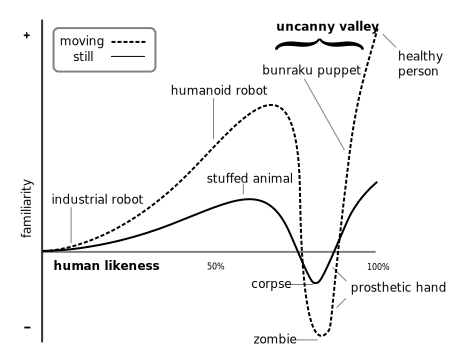
\includegraphics[width=0.5\textwidth]{Mori_Uncanny_Valley}
    \caption{Uncanny Valley}
    \label{fig:uncannyValley}
\end{center}
\end{figure}

The reason behind the uncanny valley is a  a switch of perception mechanism.
For the unfamiliar, the perception mechanism is based on analogy,
where the the identification of qualitative properties plays the major role.
As long as the qualitative properties is the the same with our experience, we may accept characters as ``believable''.
In this situation we are checking the Global Motor Invariant.

When the object becomes more familiar, it will trigger our experience memory.
Details are utilized to check the observation against memory,
which closely relate to the idea of Local Motor Invariant.


A object that has desired qualitative property may not have the quantitative details for quantitative perception mechanism.
When the switch of mechanism results in a drop in likeness.
This proposal is bold and early, but might be a worthwhile topic for further biological and physiological research.





%%% ----------------------------------------------------------------------

% ------------------------------------------------------------------------

%%% Local Variables: 
%%% mode: latex
%%% TeX-master: "../thesis"
%%% End: 
